\documentclass{standalone}
\usepackage{tikz}
\usetikzlibrary{positioning, fit, shapes, intersections}

\begin{document}

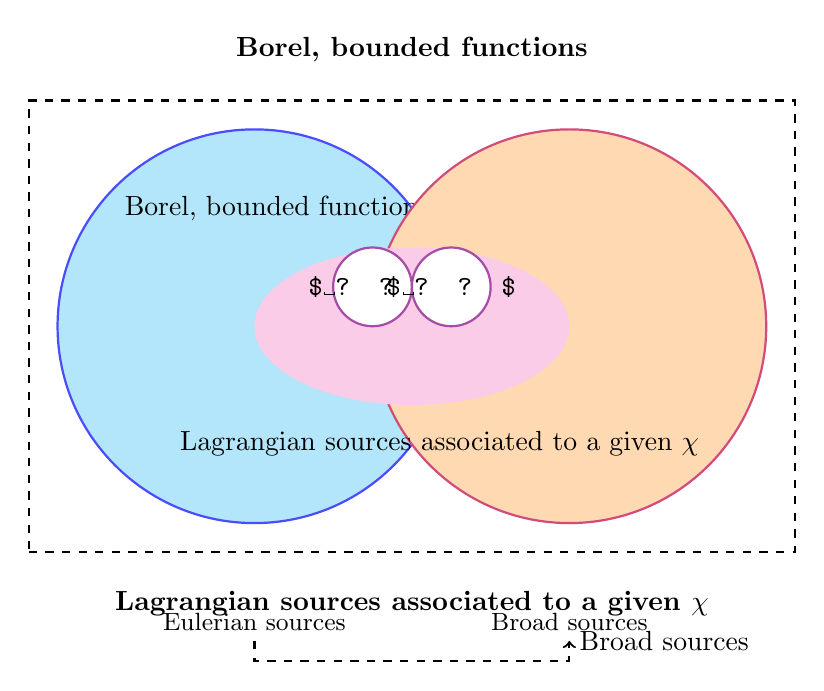
\begin{tikzpicture}[thick]

% Define the main shapes
\node[circle, draw=blue!70, fill=cyan!30, minimum width=5cm, label={[anchor=north west]north west:Borel, bounded functions}] (A) at (-2,0) {};
\node[circle, draw=purple!70, fill=orange!30, minimum width=5cm, label={[anchor=south east]south east:Lagrangian sources associated to a given $\chi$}] (B) at (2,0) {};

% Draw the intersection area (ellipse)
\node[draw=none, ellipse, fill=magenta!20, inner sep=0pt, minimum width=4cm, minimum height=2cm, anchor=center] (intersection) at (0,0) {};

% Add text inside the intersection area
\node[circle, draw=violet!70, fill=white, minimum size=1cm, label={center:\texttt{\textdollar\textvisiblespace ? ? \textdollar}}] (source1) at (-0.5,0.5) {};
\node[circle, draw=violet!70, fill=white, minimum size=1cm, label={center:\texttt{\textdollar\textvisiblespace ? ? \textdollar}}] (source2) at (0.5,0.5) {};

% Add labels outside the circles
\node[below=of A, align=center, font=\small] (eulerian_label) {Eulerian sources};
\node[below=of B, align=center, font=\small] (lagrangian_label) {Broad sources};

% Draw a rectangle around everything
\node[draw=black, dashed, inner sep=10pt, fit=(A)(B)(intersection), label={[font=\bfseries, above=10pt]north:Borel, bounded functions}, label={[font=\bfseries, below=10pt]south:Lagrangian sources associated to a given $\chi$}] (frame) {};

% Connect Eulerian and Broad sources
\draw[dashed, ->] (eulerian_label) -- ++(0,-0.5) -| node[above right]{Broad sources} (lagrangian_label);

\end{tikzpicture}

\end{document}